\begin{thms}
	Modellbildung der Strecke durch mathematische Beschreibungen der Wirkungszusammenh�nge zwischen den Systemgr��en, die f�r die Aufgabenstellung relevant sind.
\end{thms}

Ein Modell ist eine aufgabenspezifische Vereinfachung der Realit�t. In der RT bew�hrte Modellierungsform:

\section{Darstellung der Strecke als Strukturbild (Blockschaltbild)}
\subsection{Beispiel: Permant erregter Gleichstrommotor}
\begin{itemize}
	\item Ger�teschema: (siehe Beiblatt 4)
	\item Systemdarstellung:
\end{itemize}

\begin{center}
	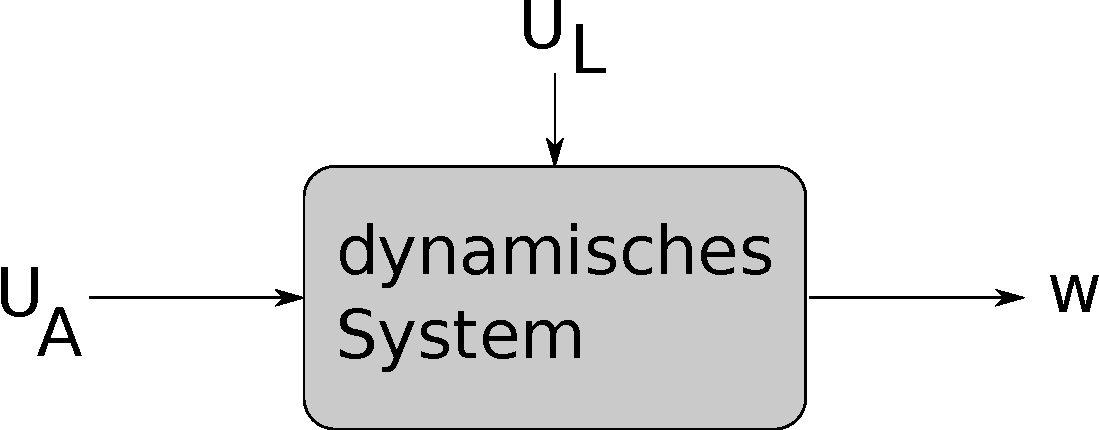
\includegraphics[width=200px]{graphics/gleichstrommotor.pdf}
\end{center}

\subsubsection{Ermittlung der beschreibenden Gleichungen:}

  \[u_l(t) = L \frac{di_A(t)} {dt} \longrightarrow \frac{d i_A(t)}{dt} = \frac{1}{L_A} u_l(t) \]
\begin{equation}
   \xrightarrow {\text{Integration von 0 bis t}} i_A(t) = i_A(0) + \frac{1}{L_A} \int_0^t u_l(\tau), d \tau 
\end{equation}
 \[u_A(t) = u_R + u_L + u_{ind} \]
\begin{equation}
\longrightarrow u_L(t) = u_A(t) - u_R(t) - u_{ind}(t)
\end{equation}

\begin{equation}
 u_R(t) = R_A i_A(t)
\end{equation}

\begin{equation}
 u_{ind}(t) = c \phi_F \omega(t)
\end{equation}

\subsubsection*{Rotierender Anker + Welle:}
\[J\dot{\omega} = M_\Sigma
\longrightarrow \dot{\omega} = \frac{1}{J} M_\Sigma(t) \]
\begin{equation}
 \xrightarrow {\text{Integration von 0 bis t}}  \omega(t) = \omega(0) + \frac{1}{J} \int_0^t M_z(\tau), d \tau
\end{equation}

		\begin{center}
			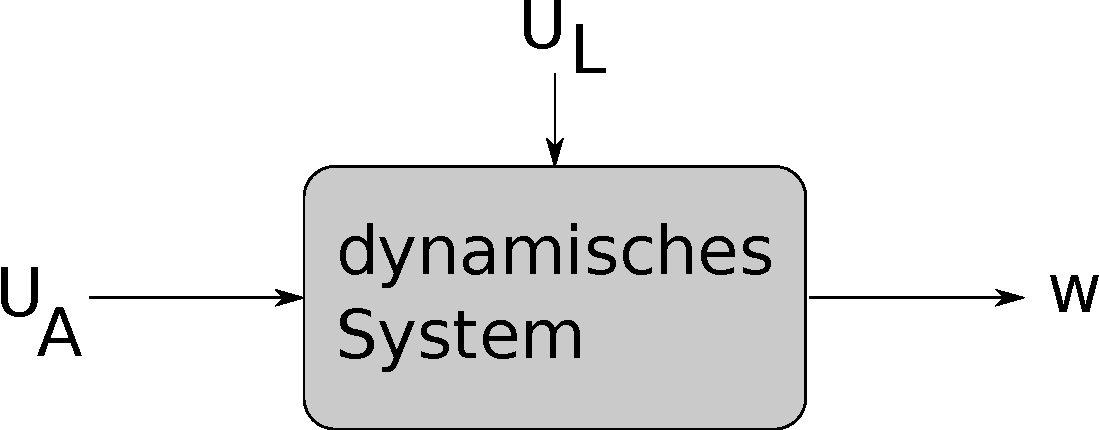
\includegraphics[width=200px]{graphics/gleichstrommotor.pdf}
		\end{center}
\begin{itemize}
		\item Ermittlung der beschreibenden Gleichungen:
		\subitem Ankerstromkreis
		\begin{align}
		u_L=L\frac{di_A}{dt} \rightarrow \frac{di_A(t)}{dt}=\frac{1}{L}u_L(t) \stackrel{\int_0^t}{\rightarrow}i_A(t)=i_A(0)+\frac{1}{L_A}\int_0^t u_L(\tau)d\tau \\
		u_A=u_R+u_L+u_{ind} \rightarrow u_L(t)=u_A(t)-u_R(t)-u_{ind}(t) \\
		u_R(t)=R_Ai_A(t) \\
		U_{ind}=c\phi\omega(t)
		\end{align}
		\subitem Rotierender Anker und Welle
		\begin{align}
		J\dot{\omega}=M_{\sum} \rightarrow \dot{\omega}(t)=\frac{1}{J}M_{\sum}(t)\stackrel{\int_0^t}{\rightarrow}\omega(t)=\omega(0)+\frac{1}{J}\int_0^t M_{\sum}(\tau)d\tau \\
		M_{\sum}(t)=M_A(t)-M_L(t) \\
		M_A(t) = c \phi_F L_A(t)
		\end{align}
	\item �bersetzung der Gleichungen ins Strukturbild {TODO:BILD}
	\begin{thms}
		Strukturbild = Graphische Darstellung der Systemregeln (durch Bl�cke und Wirkungslinien). Dadurch anschaulich und \underline{Wirkungsrichtungen} sofort ersichtlich.
	\end{thms}
\end{itemize}

\subsection{Die Bausteine des Strukturfeldes}
\begin{itemize}
	\item \underline{gerichtete Linien} geben die \underline{Systemgr��en im Zeitbereich} und ihre Wirkrichtungen wieder
	\item \underline{Bl�cke, Rechtecke und Kreise} beschreiben die Funktionsbeziehung zwischen den Systemgr��en und ordnen jedem Zeitverlauf der Eingangsgr��en
eindeutig einem Zeitverlauf der Ausgangsgr��e zu. \\
	$ \rightarrow {\text{Jeder Block wirkt als \underline{�bertragungsglied} (�G)}} $

\end{itemize}

\subsubsection{Darstellungsm�glichkeiten}
\begin{itemize}
 \item mittels Zuordnungsvorschrift \\
	bzw. Systemoperator $\boldsymbol{\mathcal{S}}$ \\
	vgl. obiges Beispiel \\
	TODO: Blockdiagram
	$ y(t) = \mathcal{S}\left \{ u(t)  \right \}$
 \item bei LZI-�G weiterhin
	\subitem mittels �bertragunsfunktion �G \\
		TODO: Blockdiagram \\
		$ y(t) \multimapdotbothA Y(s) = G(s)U(s)$
	\subitem mittels Sprungantwort $y_\sigma(t)$ \\
		(= $ y(t) $ f�r	$ u(t) $ = Einheitsprung $ \sigma(t) $ \\
		TODO: Blockdiagram \\
		$ y(t) = g(t)*u(t)  = {\dot{y}_\sigma(t)} * u(t) $\\
		(da $g(t) = {\dot{y}_\sigma(t)} $ gilt)
\item Zusammenstellung elementarer �G \\
	(nicht in noch einfachere Bestandteile zerlegbar):\\(siehe Beiblatt 5)
	
\end{itemize}

\subsubsection{\underline{Hinweise zum Totzeitglied:}}
\begin{itemize}
 \item typisch f�r Transportprozesse
 \item �F rational approximierbar z.B. gem��
      \[ e^{-T_t s} \approx \frac{1- 0,5 T_t s}{1 + 0,5 T_t s} \]
\end{itemize}

\subsubsection{H�ufig auftretende Kombinationen elementarer �G werden zu \underline{zusammengesetzten} �G zusammengefasst}
$\rightarrow$ siehe Beiblatt 6

\subsubsection{Aufbau des $PT_1$ - Gliedes aus elementaren �G:}
    \[ T\dot{y} + y = Ku \\
    \rightarrow \dot{y} = \frac{1}{T} (K u - y) = \frac{K}{T} (u - \frac{1}{K} y) \\
     \]
    \[y(t) = y(0) + \frac{K}{T} \int_0^t v(\tau) d\tau   \text{ mit } v(t) = u(t) - \frac{1}{K} y(t)
    \]
    \\
    TODO: Blockschaltbild

\subsubsection{Normierte $PT_2$-Sprungantworten f�r $D\le 1$}
$\rightarrow$ siehe Beiblatt 7




